\documentclass[12pt, a4paper]{article}
\usepackage{../notesheets}

%%%%%%%%%%%%%%%%%%%%%%%%%%%%%%%%%%%%%%%%%%%%%%%%%%
\author{Math 1210}
\title{Notesheet. Section 4.4+4.5: Optimization}
\date{}

\begin{document}
\maketitle
\nameline
%%%%%%%%%%%%%%%%%%%%%%%%%%%%%%%%%%%%%%%%%%%%%%%%%%
\begin{defi}
  Let \(f\) be a function. Then, we say a value \(f(c)\) is an
  \de{absolute maximum value} (or \de{global maximum value}) of \(f\) if
\end{defi}
\begin{thrm}
  If \(f\) is continuous on a closed interval \([a,b]\), then \(f\)
  acheives an absolute maximum value and an absolute minimum value on
  \([a,b]\).
\end{thrm}
\vspace{-1in}
\begin{ex}
  Find the absolute maximum and minimum values of the function \[
    f(x) = x^3 - 3x^2 + 1, \hspace{1in} -\frac{1}{2} \leq x \leq 4
  \]
\end{ex}
\vspace{-0.75in}
\begin{ex}
  A manufacturer of tennis rackets find that the total cost \(C(x)\)
  (in dollars) of manufacturing \(x\) rackets/day is given by \(C(x) =
  400 + 4x + 0.0001x^2\). Each racket can be sold at a price of \(p\)
  dollars, where \(p\) is related to \(x\) by the demand equation \(p
  = 10 - 0.0004x\). If all rackets that are manufactured can be sold,
  find the daily level of production that will yield a maximum profit
  for the manufacturer. (Hint: \(\sqrt{15} \approx 3.9\)).
\end{ex}
\begin{ex}
  Find the global minimum and maximum of \(f(x) = |x-3|\) on
  \([1,4]\).
\end{ex}
\begin{ex}
  % This problem comes from one of Andrew Kobin's practice worksheets on GTA resources
  Find the point on the parabola \(y = x^2+1\) that is closest to the
  point \((0,2)\).
\end{ex}
\begin{ex}
  A woman launches her boat from point \(A\) on a bank of a straight
  river, \(1\) km wide, and wants to reach point \(B\), \(10\)km
  downstream on the opposite bank, as quickly as possible. She could
  row her boat directly across the river to point \(C\) and then run
  to \(B\), or she could row directly to \(B\), or she could row to
  some point \(D\) between \(C\) and \(B\), and then run to \(B\). If
  she can row \(6\) km/h and run \(10\) km/h, where should she land to
  reach \(B\) as soon as possible? (We assume that the speed of the
  water is negligible compared with the speed at which the woman
  rows.) Hint: \(\frac{5}{24} \approx 0.20833, \frac{37}{40} =
  0.925\), and \(\sqrt{101} \approx 10.05\). \\
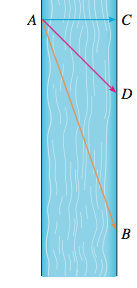
\includegraphics[scale=0.5]{images/river}
\end{ex}
\vspace{-1.5in}
\begin{ex}
  A grain silo has the shape of a right circular cylinder surmounted
  by a hemisphere (and the silo has no base). If the silo is to have a capacity of \(504 \pi
  \text{ ft}^3\), find the radius and height of the silo that requires
  the least amount of material to construct.\\
  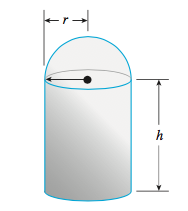
\includegraphics[scale=0.6]{images/silo}
\end{ex}
%%%%%%%%%%%%%%%%%%%%%%%%%%%%%%%%%%%%%%%%%%%%%%%%%%
\end{document}
